\documentclass[../tex_main/NEMO_manual]{subfiles}
\begin{document}
% ================================================================
% Chapter — Lateral Boundary Condition (LBC) 
% ================================================================
\chapter{Lateral Boundary Condition (LBC)}
\label{chap:LBC}
\minitoc

\newpage
$\ $\newline    % force a new ligne


%gm% add here introduction to this chapter

% ================================================================
% Boundary Condition at the Coast
% ================================================================
\section{Boundary condition at the coast (\protect\np{rn\_shlat})}
\label{sec:LBC_coast}
%--------------------------------------------nam_lbc-------------------------------------------------------
\forfile{../namelists/namlbc} 
%--------------------------------------------------------------------------------------------------------------

%The lateral ocean boundary conditions contiguous to coastlines are Neumann conditions for heat and salt (no flux across boundaries) and Dirichlet conditions for momentum (ranging from free-slip to "strong" no-slip). They are handled automatically by the mask system (see \autoref{subsec:DOM_msk}). 

%OPA allows land and topography grid points in the computational domain due to the presence of continents or islands, and includes the use of a full or partial step representation of bottom topography. The computation is performed over the whole domain, i.e. we do not try to restrict the computation to ocean-only points. This choice has two motivations. Firstly, working on ocean only grid points overloads the code and harms the code readability. Secondly, and more importantly, it drastically reduces the vector portion of the computation, leading to a dramatic increase of CPU time requirement on vector computers.  The current section describes how the masking affects the computation of the various terms of the equations with respect to the boundary condition at solid walls. The process of defining which areas are to be masked is described in \autoref{subsec:DOM_msk}.

Options are defined through the \ngn{namlbc} namelist variables.
The discrete representation of a domain with complex boundaries (coastlines and 
bottom topography) leads to arrays that include large portions where a computation 
is not required as the model variables remain at zero. Nevertheless, vectorial 
supercomputers are far more efficient when computing over a whole array, and the 
readability of a code is greatly improved when boundary conditions are applied in 
an automatic way rather than by a specific computation before or after each 
computational loop. An efficient way to work over the whole domain while specifying 
the boundary conditions, is to use multiplication by mask arrays in the computation. 
A mask array is a matrix whose elements are $1$ in the ocean domain and $0$ 
elsewhere. A simple multiplication of a variable by its own mask ensures that it will 
remain zero over land areas. Since most of the boundary conditions consist of a 
zero flux across the solid boundaries, they can be simply applied by multiplying 
variables by the correct mask arrays, $i.e.$ the mask array of the grid point where 
the flux is evaluated. For example, the heat flux in the \textbf{i}-direction is evaluated 
at $u$-points. Evaluating this quantity as,

\begin{equation} \label{eq:lbc_aaaa}
\frac{A^{lT} }{e_1 }\frac{\partial T}{\partial i}\equiv \frac{A_u^{lT} 
}{e_{1u} } \; \delta _{i+1 / 2} \left[ T \right]\;\;mask_u 
\end{equation}
(where mask$_{u}$ is the mask array at a $u$-point) ensures that the heat flux is 
zero inside land and at the boundaries, since mask$_{u}$ is zero at solid boundaries 
which in this case are defined at $u$-points (normal velocity $u$ remains zero at 
the coast) (\autoref{fig:LBC_uv}). 

%>>>>>>>>>>>>>>>>>>>>>>>>>>>>
\begin{figure}[!t]     \begin{center}
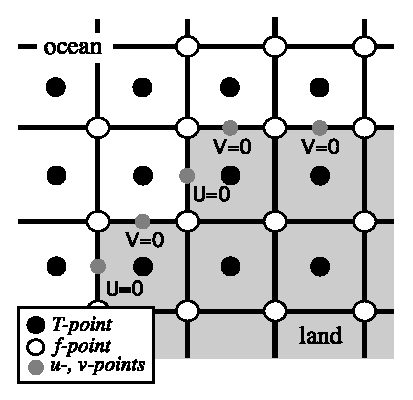
\includegraphics[width=0.90\textwidth]{Fig_LBC_uv}
\caption{  \protect\label{fig:LBC_uv}
Lateral boundary (thick line) at T-level. The velocity normal to the boundary is set to zero.}
\end{center}   \end{figure}
%>>>>>>>>>>>>>>>>>>>>>>>>>>>>

For momentum the situation is a bit more complex as two boundary conditions 
must be provided along the coast (one each for the normal and tangential velocities). 
The boundary of the ocean in the C-grid is defined by the velocity-faces. 
For example, at a given $T$-level, the lateral boundary (a coastline or an intersection 
with the bottom topography) is made of segments joining $f$-points, and normal 
velocity points are located between two $f-$points (\autoref{fig:LBC_uv}). 
The boundary condition on the normal velocity (no flux through solid boundaries) 
can thus be easily implemented using the mask system. The boundary condition 
on the tangential velocity requires a more specific treatment. This boundary 
condition influences the relative vorticity and momentum diffusive trends, and is 
required in order to compute the vorticity at the coast. Four different types of 
lateral boundary condition are available, controlled by the value of the \np{rn\_shlat} 
namelist parameter. (The value of the mask$_{f}$ array along the coastline is set 
equal to this parameter.) These are:

%>>>>>>>>>>>>>>>>>>>>>>>>>>>>
\begin{figure}[!p] \begin{center}
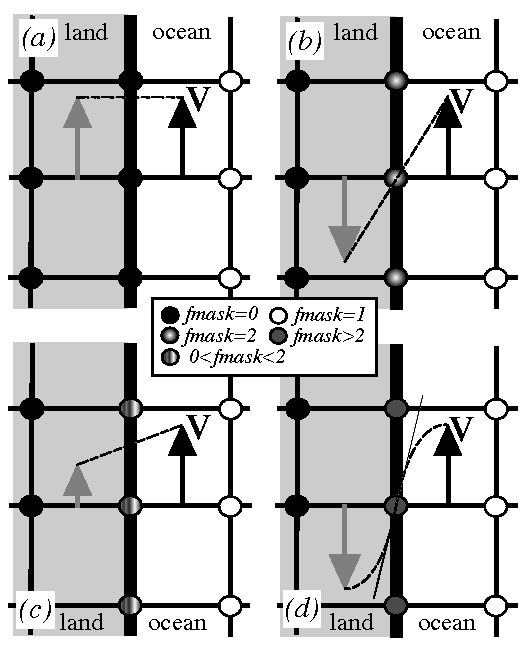
\includegraphics[width=0.90\textwidth]{Fig_LBC_shlat}
\caption{     \protect\label{fig:LBC_shlat} 
lateral boundary condition (a) free-slip ($rn\_shlat=0$) ; (b) no-slip ($rn\_shlat=2$) 
; (c) "partial" free-slip ($0<rn\_shlat<2$) and (d) "strong" no-slip ($2<rn\_shlat$). 
Implied "ghost" velocity inside land area is display in grey. }
\end{center}    \end{figure}
%>>>>>>>>>>>>>>>>>>>>>>>>>>>>

\begin{description}

\item[free-slip boundary condition (\np{rn\_shlat}\forcode{ = 0}): ]  the tangential velocity at the 
coastline is equal to the offshore velocity, $i.e.$ the normal derivative of the 
tangential velocity is zero at the coast, so the vorticity: mask$_{f}$ array is set 
to zero inside the land and just at the coast (\autoref{fig:LBC_shlat}-a).

\item[no-slip boundary condition (\np{rn\_shlat}\forcode{ = 2}): ] the tangential velocity vanishes 
at the coastline. Assuming that the tangential velocity decreases linearly from 
the closest ocean velocity grid point to the coastline, the normal derivative is 
evaluated as if the velocities at the closest land velocity gridpoint and the closest 
ocean velocity gridpoint were of the same magnitude but in the opposite direction 
(\autoref{fig:LBC_shlat}-b). Therefore, the vorticity along the coastlines is given by: 

\begin{equation*}
\zeta \equiv 2 \left(\delta_{i+1/2} \left[e_{2v} v \right] - \delta_{j+1/2} \left[e_{1u} u \right] \right) / \left(e_{1f} e_{2f} \right) \ ,
\end{equation*}
where $u$ and $v$ are masked fields. Setting the mask$_{f}$ array to $2$ along 
the coastline provides a vorticity field computed with the no-slip boundary condition, 
simply by multiplying it by the mask$_{f}$ :
\begin{equation} \label{eq:lbc_bbbb}
\zeta \equiv \frac{1}{e_{1f} {\kern 1pt}e_{2f} }\left( {\delta _{i+1/2} 
\left[ {e_{2v} \,v} \right]-\delta _{j+1/2} \left[ {e_{1u} \,u} \right]} 
\right)\;\mbox{mask}_f 
\end{equation}

\item["partial" free-slip boundary condition (0$<$\np{rn\_shlat}$<$2): ] the tangential 
velocity at the coastline is smaller than the offshore velocity, $i.e.$ there is a lateral 
friction but not strong enough to make the tangential velocity at the coast vanish 
(\autoref{fig:LBC_shlat}-c). This can be selected by providing a value of mask$_{f}$ 
strictly inbetween $0$ and $2$.

\item["strong" no-slip boundary condition (2$<$\np{rn\_shlat}): ] the viscous boundary 
layer is assumed to be smaller than half the grid size (\autoref{fig:LBC_shlat}-d). 
The friction is thus larger than in the no-slip case.

\end{description}

Note that when the bottom topography is entirely represented by the $s$-coor-dinates 
(pure $s$-coordinate), the lateral boundary condition on tangential velocity is of much 
less importance as it is only applied next to the coast where the minimum water depth 
can be quite shallow.


% ================================================================
% Boundary Condition around the Model Domain
% ================================================================
\section{Model domain boundary condition (\protect\np{jperio})}
\label{sec:LBC_jperio}

At the model domain boundaries several choices are offered: closed, cyclic east-west, 
south symmetric across the equator, a north-fold, and combination closed-north fold 
or cyclic-north-fold. The north-fold boundary condition is associated with the 3-pole ORCA mesh. 

% -------------------------------------------------------------------------------------------------------------
%        Closed, cyclic, south symmetric (\np{jperio}\forcode{ = 0..2}) 
% -------------------------------------------------------------------------------------------------------------
\subsection{Closed, cyclic, south symmetric (\protect\np{jperio}\forcode{= 0..2})}
\label{subsec:LBC_jperio012}

The choice of closed, cyclic or symmetric model domain boundary condition is made 
by setting \np{jperio} to 0, 1 or 2 in namelist \ngn{namcfg}. Each time such a boundary 
condition is needed, it is set by a call to routine \mdl{lbclnk}. The computation of 
momentum and tracer trends proceeds from $i=2$ to $i=jpi-1$ and from $j=2$ to 
$j=jpj-1$, $i.e.$ in the model interior. To choose a lateral model boundary condition 
is to specify the first and last rows and columns of the model variables. 

\begin{description}

\item[For closed boundary (\np{jperio}\forcode{ = 0})], solid walls are imposed at all model 
boundaries: first and last rows and columns are set to zero.

\item[For cyclic east-west boundary (\np{jperio}\forcode{ = 1})], first and last rows are set 
to zero (closed) whilst the first column is set to the value of the last-but-one column 
and the last column to the value of the second one (\autoref{fig:LBC_jperio}-a). 
Whatever flows out of the eastern (western) end of the basin enters the western 
(eastern) end. Note that there is no option for north-south cyclic or for doubly 
cyclic cases.

\item[For symmetric boundary condition across the equator (\np{jperio}\forcode{ = 2})], 
last rows, and first and last columns are set to zero (closed). The row of symmetry 
is chosen to be the $u$- and $T-$points equator line ($j=2$, i.e. at the southern 
end of the domain). For arrays defined at $u-$ or $T-$points, the first row is set 
to the value of the third row while for most of $v$- and $f$-point arrays ($v$, $\zeta$, 
$j\psi$, but \gmcomment{not sure why this is "but"} scalar arrays such as eddy coefficients) 
the first row is set to minus the value of the second row (\autoref{fig:LBC_jperio}-b). 
Note that this boundary condition is not yet available for the case of a massively 
parallel computer (\textbf{key{\_}mpp} defined).

\end{description}

%>>>>>>>>>>>>>>>>>>>>>>>>>>>>
\begin{figure}[!t]     \begin{center}
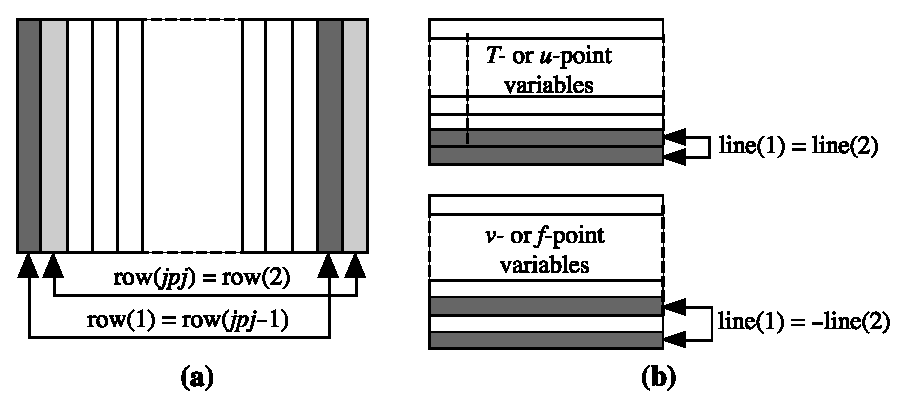
\includegraphics[width=1.0\textwidth]{Fig_LBC_jperio}
\caption{    \protect\label{fig:LBC_jperio}
setting of (a) east-west cyclic  (b) symmetric across the equator boundary conditions.}
\end{center}   \end{figure}
%>>>>>>>>>>>>>>>>>>>>>>>>>>>>

% -------------------------------------------------------------------------------------------------------------
%        North fold (\textit{jperio = 3 }to $6)$ 
% -------------------------------------------------------------------------------------------------------------
\subsection{North-fold (\protect\np{jperio}\forcode{ = 3..6})}
\label{subsec:LBC_north_fold}

The north fold boundary condition has been introduced in order to handle the north 
boundary of a three-polar ORCA grid. Such a grid has two poles in the northern hemisphere 
(\autoref{fig:MISC_ORCA_msh}, and thus requires a specific treatment illustrated in \autoref{fig:North_Fold_T}. 
Further information can be found in \mdl{lbcnfd} module which applies the north fold boundary condition.

%>>>>>>>>>>>>>>>>>>>>>>>>>>>>
\begin{figure}[!t]    \begin{center}
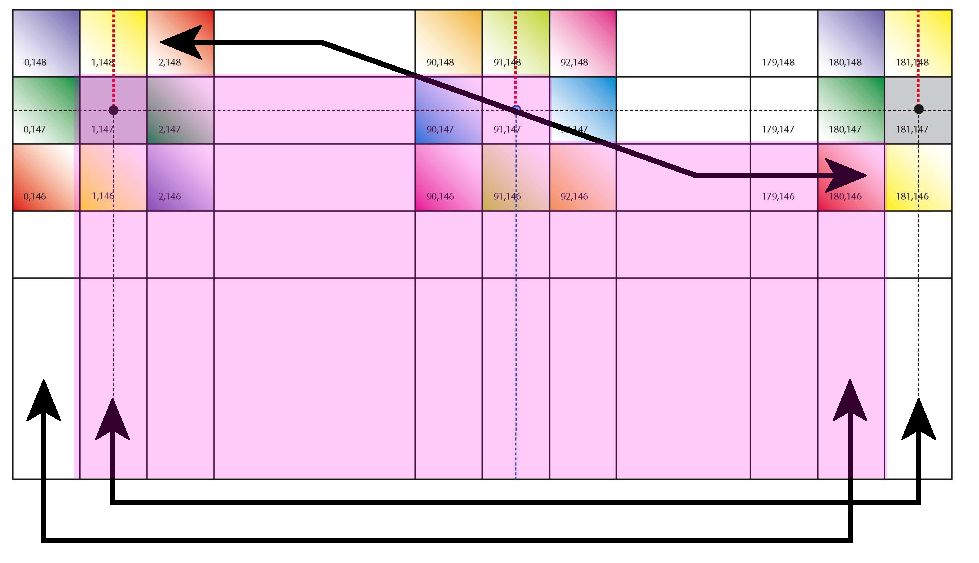
\includegraphics[width=0.90\textwidth]{Fig_North_Fold_T}
\caption{    \protect\label{fig:North_Fold_T} 
North fold boundary with a $T$-point pivot and cyclic east-west boundary condition 
($jperio=4$), as used in ORCA 2, 1/4, and 1/12. Pink shaded area corresponds 
to the inner domain mask (see text). }
\end{center}   \end{figure}
%>>>>>>>>>>>>>>>>>>>>>>>>>>>>

% ====================================================================
% Exchange with neighbouring processors 
% ====================================================================
\section{Exchange with neighbouring processors (\protect\mdl{lbclnk}, \protect\mdl{lib\_mpp})}
\label{sec:LBC_mpp}

For massively parallel processing (mpp), a domain decomposition method is used. 
The basic idea of the method is to split the large computation domain of a numerical 
experiment into several smaller domains and solve the set of equations by addressing 
independent local problems. Each processor has its own local memory and computes 
the model equation over a subdomain of the whole model domain. The subdomain 
boundary conditions are specified through communications between processors 
which are organized by explicit statements (message passing method). 

A big advantage is that the method does not need many modifications of the initial 
FORTRAN code. From the modeller's point of view, each sub domain running on 
a processor is identical to the "mono-domain" code. In addition, the programmer 
manages the communications between subdomains, and the code is faster when 
the number of processors is increased. The porting of OPA code on an iPSC860 
was achieved during Guyon's PhD [Guyon et al. 1994, 1995] in collaboration with 
CETIIS and ONERA. The implementation in the operational context and the studies 
of performance on a T3D and T3E Cray computers have been made in collaboration 
with IDRIS and CNRS. The present implementation is largely inspired by Guyon's 
work  [Guyon 1995].

The parallelization strategy is defined by the physical characteristics of the 
ocean model. Second order finite difference schemes lead to local discrete 
operators that depend at the very most on one neighbouring point. The only 
non-local computations concern the vertical physics (implicit diffusion, 
turbulent closure scheme, ...) (delocalization over the whole water column), 
and the solving of the elliptic equation associated with the surface pressure 
gradient computation (delocalization over the whole horizontal domain). 
Therefore, a pencil strategy is used for the data sub-structuration 
: the 3D initial domain is laid out on local processor 
memories following a 2D horizontal topological splitting. Each sub-domain 
computes its own surface and bottom boundary conditions and has a side 
wall overlapping interface which defines the lateral boundary conditions for 
computations in the inner sub-domain. The overlapping area consists of the 
two rows at each edge of the sub-domain. After a computation, a communication 
phase starts: each processor sends to its neighbouring processors the update 
values of the points corresponding to the interior overlapping area to its 
neighbouring sub-domain ($i.e.$ the innermost of the two overlapping rows). 
The communication is done through the Message Passing Interface (MPI). 
The data exchanges between processors are required at the very 
place where lateral domain boundary conditions are set in the mono-domain 
computation : the \rou{lbc\_lnk} routine (found in \mdl{lbclnk} module) 
which manages such conditions is interfaced with routines found in \mdl{lib\_mpp} module 
when running on an MPP computer ($i.e.$ when \key{mpp\_mpi} defined). 
It has to be pointed out that when using the MPP version of the model, 
the east-west cyclic boundary condition is done implicitly, 
whilst the south-symmetric boundary condition option is not available.

%>>>>>>>>>>>>>>>>>>>>>>>>>>>>
\begin{figure}[!t]    \begin{center}
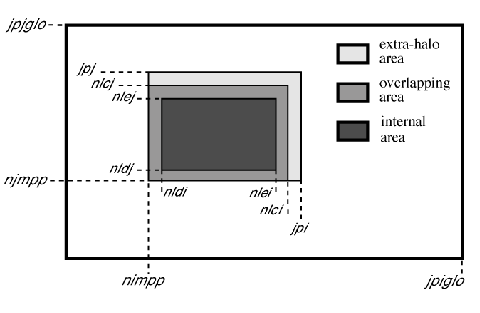
\includegraphics[width=0.90\textwidth]{Fig_mpp}
\caption{   \protect\label{fig:mpp} 
Positioning of a sub-domain when massively parallel processing is used. }
\end{center}   \end{figure}
%>>>>>>>>>>>>>>>>>>>>>>>>>>>>

In the standard version of \NEMO, the splitting is regular and arithmetic.
The i-axis is divided by \jp{jpni} and the j-axis by \jp{jpnj} for a number of processors 
\jp{jpnij} most often equal to $jpni \times jpnj$ (parameters set in 
 \ngn{nammpp} namelist). Each processor is independent and without message passing 
 or synchronous process, programs run alone and access just its own local memory. 
 For this reason, the main model dimensions are now the local dimensions of the subdomain (pencil) 
 that are named \jp{jpi}, \jp{jpj}, \jp{jpk}. These dimensions include the internal 
 domain and the overlapping rows. The number of rows to exchange (known as 
 the halo) is usually set to one (\jp{jpreci}=1, in \mdl{par\_oce}). The whole domain 
 dimensions are named \np{jpiglo}, \np{jpjglo} and \jp{jpk}. The relationship between 
 the whole domain and a sub-domain is:
\begin{eqnarray} 
      jpi & = & ( jpiglo-2*jpreci + (jpni-1) ) / jpni + 2*jpreci  \nonumber \\
      jpj & = & ( jpjglo-2*jprecj + (jpnj-1) ) / jpnj + 2*jprecj  \label{eq:lbc_jpi}
\end{eqnarray}
where \jp{jpni}, \jp{jpnj} are the number of processors following the i- and j-axis.

One also defines variables nldi and nlei which correspond to the internal domain bounds, 
and the variables nimpp and njmpp which are the position of the (1,1) grid-point in the global domain. 
An element of $T_{l}$, a local array (subdomain) corresponds to an element of $T_{g}$, 
a global array (whole domain) by the relationship: 
\begin{equation} \label{eq:lbc_nimpp}
T_{g} (i+nimpp-1,j+njmpp-1,k) = T_{l} (i,j,k),
\end{equation}
with  $1 \leq i \leq jpi$, $1  \leq j \leq jpj $ , and  $1  \leq k \leq jpk$.

Processors are numbered from 0 to $jpnij-1$, the number is saved in the variable 
nproc. In the standard version, a processor has no more than four neighbouring 
processors named nono (for north), noea (east), noso (south) and nowe (west) 
and two variables, nbondi and nbondj, indicate the relative position of the processor :
\begin{itemize}
\item 		nbondi = -1 	an east neighbour, no west processor,
\item 		nbondi =  0	an east neighbour, a west neighbour,
\item 		nbondi =  1 	no east processor, a west neighbour,
\item 		nbondi =  2 	no splitting following the i-axis.
\end{itemize}
During the simulation, processors exchange data with their neighbours. 
If there is effectively a neighbour, the processor receives variables from this 
processor on its overlapping row, and sends the data issued from internal 
domain corresponding to the overlapping row of the other processor.


The \NEMO model computes equation terms with the help of mask arrays (0 on land 
points and 1 on sea points). It is easily readable and very efficient in the context of 
a computer with vectorial architecture. However, in the case of a scalar processor, 
computations over the land regions become more expensive in terms of CPU time. 
It is worse when we use a complex configuration with a realistic bathymetry like the 
global ocean where more than 50 \% of points are land points. For this reason, a 
pre-processing tool can be used to choose the mpp domain decomposition with a 
maximum number of only land points processors, which can then be eliminated (\autoref{fig:mppini2})
(For example, the mpp\_optimiz tools, available from the DRAKKAR web site). 
This optimisation is dependent on the specific bathymetry employed. The user 
then chooses optimal parameters \jp{jpni}, \jp{jpnj} and \jp{jpnij} with 
$jpnij < jpni \times jpnj$, leading to the elimination of $jpni \times jpnj - jpnij$ 
land processors. When those parameters are specified in \ngn{nammpp} namelist, 
the algorithm in the \rou{inimpp2} routine sets each processor's parameters (nbound, 
nono, noea,...) so that the land-only processors are not taken into account. 

\gmcomment{Note that the inimpp2 routine is general so that the original inimpp 
routine should be suppressed from the code.}

When land processors are eliminated, the value corresponding to these locations in 
the model output files is undefined. Note that this is a problem for the meshmask file 
which requires to be defined over the whole domain. Therefore, user should not eliminate 
land processors when creating a meshmask file ($i.e.$ when setting a non-zero value to \np{nn\_msh}).

%>>>>>>>>>>>>>>>>>>>>>>>>>>>>
\begin{figure}[!ht]     \begin{center}
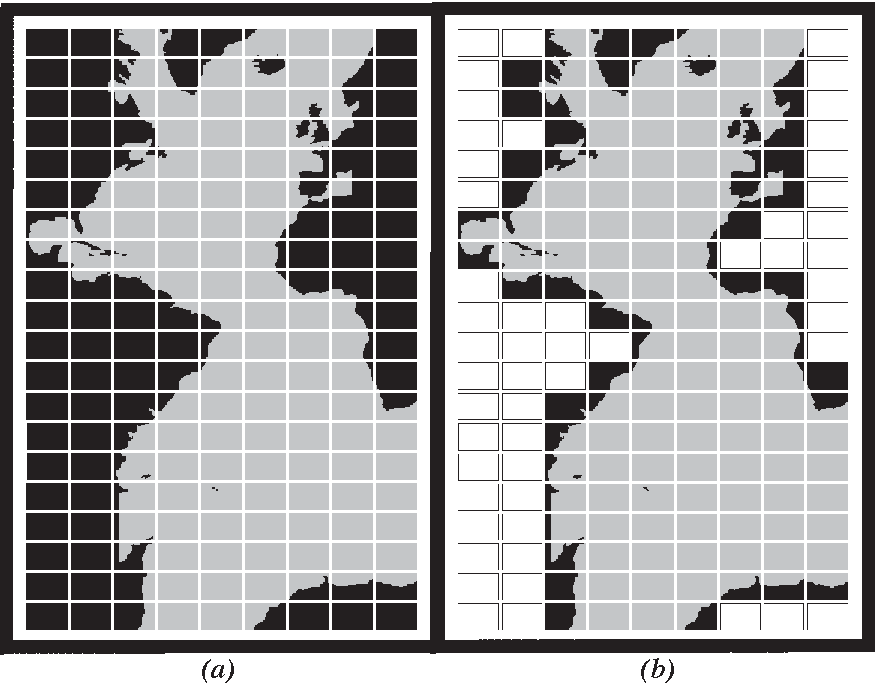
\includegraphics[width=0.90\textwidth]{Fig_mppini2}
\caption {    \protect\label{fig:mppini2}
Example of Atlantic domain defined for the CLIPPER projet. Initial grid is 
composed of 773 x 1236 horizontal points. 
(a) the domain is split onto 9 \time 20 subdomains (jpni=9, jpnj=20). 
52 subdomains are land areas. 
(b) 52 subdomains are eliminated (white rectangles) and the resulting number 
of processors really used during the computation is jpnij=128.}
\end{center}   \end{figure}
%>>>>>>>>>>>>>>>>>>>>>>>>>>>>


% ====================================================================
% Unstructured open boundaries BDY 
% ====================================================================
\section{Unstructured open boundary conditions (BDY)}
\label{sec:LBC_bdy}

%-----------------------------------------nambdy--------------------------------------------
\forfile{../namelists/nambdy} 
%-----------------------------------------------------------------------------------------------
%-----------------------------------------nambdy_index--------------------------------------------
%\forfile{../namelists/nambdy_index}
%-----------------------------------------------------------------------------------------------
%-----------------------------------------nambdy_dta--------------------------------------------
\forfile{../namelists/nambdy_dta} 
%-----------------------------------------------------------------------------------------------
%-----------------------------------------nambdy_dta--------------------------------------------
%\forfile{../namelists/nambdy_dta2} 
%-----------------------------------------------------------------------------------------------

Options are defined through the \ngn{nambdy} \ngn{nambdy\_index} 
\ngn{nambdy\_dta} \ngn{nambdy\_dta2} namelist variables.
The BDY module is the core implementation of open boundary
conditions for regional configurations. It implements the Flow
Relaxation Scheme algorithm for temperature, salinity, velocities and
ice fields, and the Flather radiation condition for the depth-mean
transports. The specification of the location of the open boundary is
completely flexible and allows for example the open boundary to follow
an isobath or other irregular contour. 

The BDY module was modelled on the OBC module (see NEMO 3.4) and shares many
features and a similar coding structure \citep{Chanut2005}.

Boundary data files used with earlier versions of NEMO may need
to be re-ordered to work with this version. See the
section on the Input Boundary Data Files for details.

%----------------------------------------------
\subsection{Namelists}
\label{subsec:BDY_namelist}

The BDY module is activated by setting \np{ln\_bdy} to true.
It is possible to define more than one boundary ``set'' and apply
different boundary conditions to each set. The number of boundary
sets is defined by \np{nb\_bdy}.  Each boundary set may be defined
as a set of straight line segments in a namelist
(\np{ln\_coords\_file}\forcode{ = .false.}) or read in from a file
(\np{ln\_coords\_file}\forcode{ = .true.}). If the set is defined in a namelist,
then the namelists nambdy\_index must be included separately, one for
each set. If the set is defined by a file, then a
``\ifile{coordinates.bdy}'' file must be provided. The coordinates.bdy file
is analagous to the usual NEMO ``\ifile{coordinates}'' file. In the example
above, there are two boundary sets, the first of which is defined via
a file and the second is defined in a namelist. For more details of
the definition of the boundary geometry see section
\autoref{subsec:BDY_geometry}.

For each boundary set a boundary
condition has to be chosen for the barotropic solution (``u2d'':
sea-surface height and barotropic velocities), for the baroclinic
velocities (``u3d''), and for the active tracers\footnote{The BDY
  module does not deal with passive tracers at this version}
(``tra''). For each set of variables there is a choice of algorithm
and a choice for the data, eg. for the active tracers the algorithm is
set by \np{nn\_tra} and the choice of data is set by
\np{nn\_tra\_dta}. 

The choice of algorithm is currently as follows:

\mbox{}

\begin{itemize}
\item[0.] No boundary condition applied. So the solution will ``see''
  the land points around the edge of the edge of the domain.
\item[1.] Flow Relaxation Scheme (FRS) available for all variables. 
\item[2.] Flather radiation scheme for the barotropic variables. The
  Flather scheme is not compatible with the filtered free surface
  ({\it dynspg\_ts}). 
\end{itemize}

\mbox{}

The main choice for the boundary data is
to use initial conditions as boundary data (\np{nn\_tra\_dta}\forcode{ = 0}) or to
use external data from a file (\np{nn\_tra\_dta}\forcode{ = 1}). For the
barotropic solution there is also the option to use tidal
harmonic forcing either by itself or in addition to other external
data. 

If external boundary data is required then the nambdy\_dta namelist
must be defined. One nambdy\_dta namelist is required for each boundary
set in the order in which the boundary sets are defined in nambdy. In
the example given, two boundary sets have been defined and so there
are two nambdy\_dta namelists. The boundary data is read in using the
fldread module, so the nambdy\_dta namelist is in the format required
for fldread. For each variable required, the filename, the frequency
of the files and the frequency of the data in the files is given. Also
whether or not time-interpolation is required and whether the data is
climatological (time-cyclic) data. Note that on-the-fly spatial
interpolation of boundary data is not available at this version. 

In the example namelists given, two boundary sets are defined. The
first set is defined via a file and applies FRS conditions to
temperature and salinity and Flather conditions to the barotropic
variables. External data is provided in daily files (from a
large-scale model). Tidal harmonic forcing is also used. The second
set is defined in a namelist. FRS conditions are applied on
temperature and salinity and climatological data is read from external
files. 

%----------------------------------------------
\subsection{Flow relaxation scheme}
\label{subsec:BDY_FRS_scheme}

The Flow Relaxation Scheme (FRS) \citep{Davies_QJRMS76,Engerdahl_Tel95},
applies a simple relaxation of the model fields to
externally-specified values over a zone next to the edge of the model
domain. Given a model prognostic variable $\Phi$ 
\begin{equation}  \label{eq:bdy_frs1}
\Phi(d) = \alpha(d)\Phi_{e}(d) + (1-\alpha(d))\Phi_{m}(d)\;\;\;\;\; d=1,N
\end{equation}
where $\Phi_{m}$ is the model solution and $\Phi_{e}$ is the specified
external field, $d$ gives the discrete distance from the model
boundary  and $\alpha$ is a parameter that varies from $1$ at $d=1$ to
a small value at $d=N$. It can be shown that this scheme is equivalent
to adding a relaxation term to the prognostic equation for $\Phi$ of
the form:
\begin{equation}  \label{eq:bdy_frs2}
-\frac{1}{\tau}\left(\Phi - \Phi_{e}\right)
\end{equation}
where the relaxation time scale $\tau$ is given by a function of
$\alpha$ and the model time step $\Delta t$:
\begin{equation}  \label{eq:bdy_frs3}
\tau = \frac{1-\alpha}{\alpha}  \,\rdt
\end{equation}
Thus the model solution is completely prescribed by the external
conditions at the edge of the model domain and is relaxed towards the
external conditions over the rest of the FRS zone. The application of
a relaxation zone helps to prevent spurious reflection of outgoing
signals from the model boundary. 

The function $\alpha$ is specified as a $tanh$ function:
\begin{equation}  \label{eq:bdy_frs4}
\alpha(d) = 1 - \tanh\left(\frac{d-1}{2}\right),       \quad d=1,N
\end{equation}
The width of the FRS zone is specified in the namelist as 
\np{nn\_rimwidth}. This is typically set to a value between 8 and 10. 

%----------------------------------------------
\subsection{Flather radiation scheme}
\label{subsec:BDY_flather_scheme}

The \citet{Flather_JPO94} scheme is a radiation condition on the normal, depth-mean
transport across the open boundary. It takes the form
\begin{equation}  \label{eq:bdy_fla1}
U = U_{e} + \frac{c}{h}\left(\eta - \eta_{e}\right),
\end{equation}
where $U$ is the depth-mean velocity normal to the boundary and $\eta$
is the sea surface height, both from the model. The subscript $e$
indicates the same fields from external sources. The speed of external
gravity waves is given by $c = \sqrt{gh}$, and $h$ is the depth of the
water column. The depth-mean normal velocity along the edge of the
model domain is set equal to the
external depth-mean normal velocity, plus a correction term that
allows gravity waves generated internally to exit the model boundary.
Note that the sea-surface height gradient in \autoref{eq:bdy_fla1}
is a spatial gradient across the model boundary, so that $\eta_{e}$ is
defined on the $T$ points with $nbr=1$ and $\eta$ is defined on the
$T$ points with $nbr=2$. $U$ and $U_{e}$ are defined on the $U$ or
$V$ points with $nbr=1$, $i.e.$ between the two $T$ grid points.

%----------------------------------------------
\subsection{Boundary geometry}
\label{subsec:BDY_geometry}

Each open boundary set is defined as a list of points. The information
is stored in the arrays $nbi$, $nbj$, and $nbr$ in the $idx\_bdy$
structure.  The $nbi$ and $nbj$ arrays
define the local $(i,j)$ indices of each point in the boundary zone
and the $nbr$ array defines the discrete distance from the boundary
with $nbr=1$ meaning that the point is next to the edge of the
model domain and $nbr>1$ showing that the point is increasingly
further away from the edge of the model domain. A set of $nbi$, $nbj$,
and $nbr$ arrays is defined for each of the $T$, $U$ and $V$
grids. Figure \autoref{fig:LBC_bdy_geom} shows an example of an irregular
boundary. 

The boundary geometry for each set may be defined in a namelist
nambdy\_index or by reading in a ``\ifile{coordinates.bdy}'' file. The
nambdy\_index namelist defines a series of straight-line segments for
north, east, south and west boundaries. For the northern boundary,
\np{nbdysegn} gives the number of segments, \np{jpjnob} gives the $j$
index for each segment and \np{jpindt} and \np{jpinft} give the start
and end $i$ indices for each segment with similar for the other
boundaries. These segments define a list of $T$ grid points along the
outermost row of the boundary ($nbr\,=\, 1$). The code deduces the $U$ and
$V$ points and also the points for $nbr\,>\, 1$ if
$nn\_rimwidth\,>\,1$.

The boundary geometry may also be defined from a
``\ifile{coordinates.bdy}'' file. Figure \autoref{fig:LBC_nc_header}
gives an example of the header information from such a file. The file
should contain the index arrays for each of the $T$, $U$ and $V$
grids. The arrays must be in order of increasing $nbr$. Note that the
$nbi$, $nbj$ values in the file are global values and are converted to
local values in the code. Typically this file will be used to generate
external boundary data via interpolation and so will also contain the
latitudes and longitudes of each point as shown. However, this is not
necessary to run the model. 

For some choices of irregular boundary the model domain may contain
areas of ocean which are not part of the computational domain. For
example if an open boundary is defined along an isobath, say at the
shelf break, then the areas of ocean outside of this boundary will
need to be masked out. This can be done by reading a mask file defined
as \np{cn\_mask\_file} in the nam\_bdy namelist. Only one mask file is
used even if multiple boundary sets are defined.

%>>>>>>>>>>>>>>>>>>>>>>>>>>>>
\begin{figure}[!t]      \begin{center}
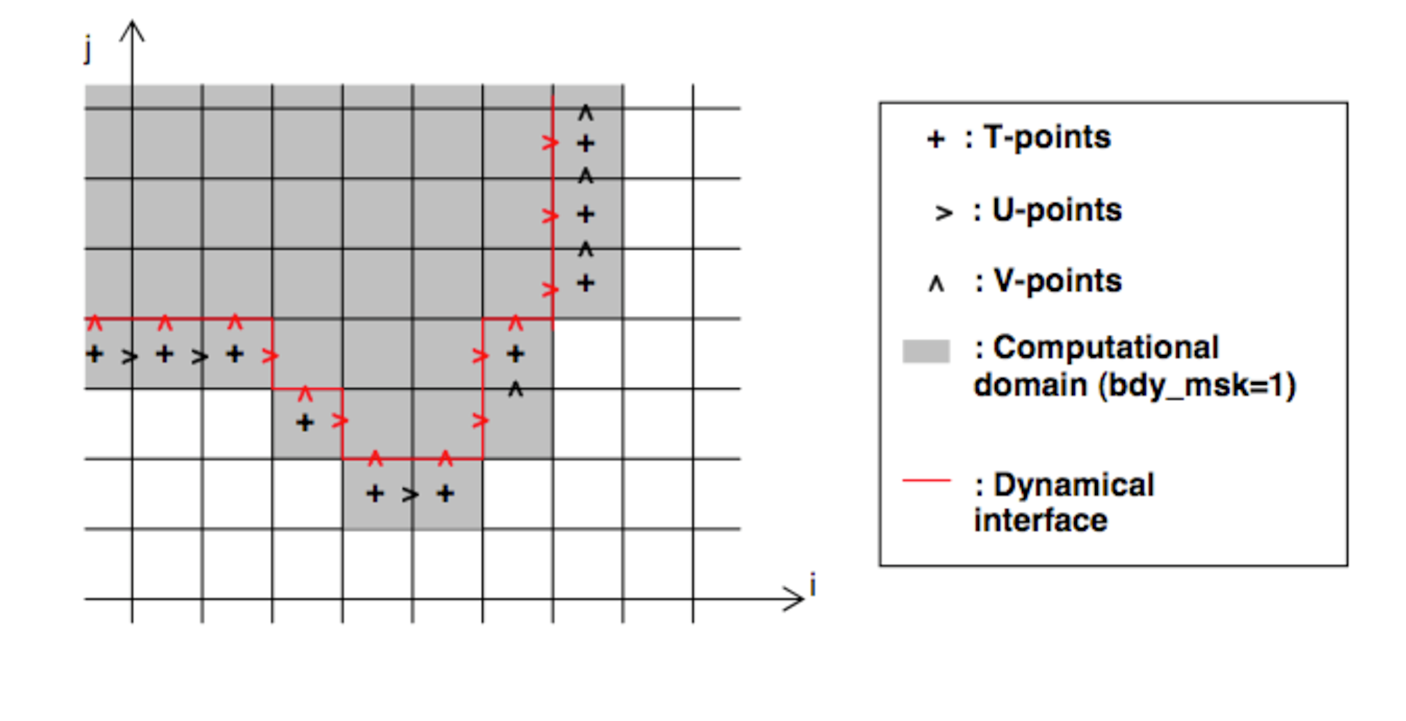
\includegraphics[width=1.0\textwidth]{Fig_LBC_bdy_geom}
\caption {      \protect\label{fig:LBC_bdy_geom}
Example of geometry of unstructured open boundary}
\end{center}   \end{figure}
%>>>>>>>>>>>>>>>>>>>>>>>>>>>>

%----------------------------------------------
\subsection{Input boundary data files}
\label{subsec:BDY_data}

The data files contain the data arrays
in the order in which the points are defined in the $nbi$ and $nbj$
arrays. The data arrays are dimensioned on: a time dimension;
$xb$ which is the index of the boundary data point in the horizontal;
and $yb$ which is a degenerate dimension of 1 to enable the file to be
read by the standard NEMO I/O routines. The 3D fields also have a
depth dimension. 

At Version 3.4 there are new restrictions on the order in which the
boundary points are defined (and therefore restrictions on the order
of the data in the file). In particular:

\mbox{}

\begin{enumerate}
\item The data points must be in order of increasing $nbr$, ie. all
  the $nbr=1$ points, then all the $nbr=2$ points etc.
\item All the data for a particular boundary set must be in the same
  order. (Prior to 3.4 it was possible to define barotropic data in a
  different order to the data for tracers and baroclinic velocities). 
\end{enumerate}

\mbox{}

These restrictions mean that data files used with previous versions of
the model may not work with version 3.4. A fortran utility
{\it bdy\_reorder} exists in the TOOLS directory which will re-order the
data in old BDY data files. 

%>>>>>>>>>>>>>>>>>>>>>>>>>>>>
\begin{figure}[!t]     \begin{center}
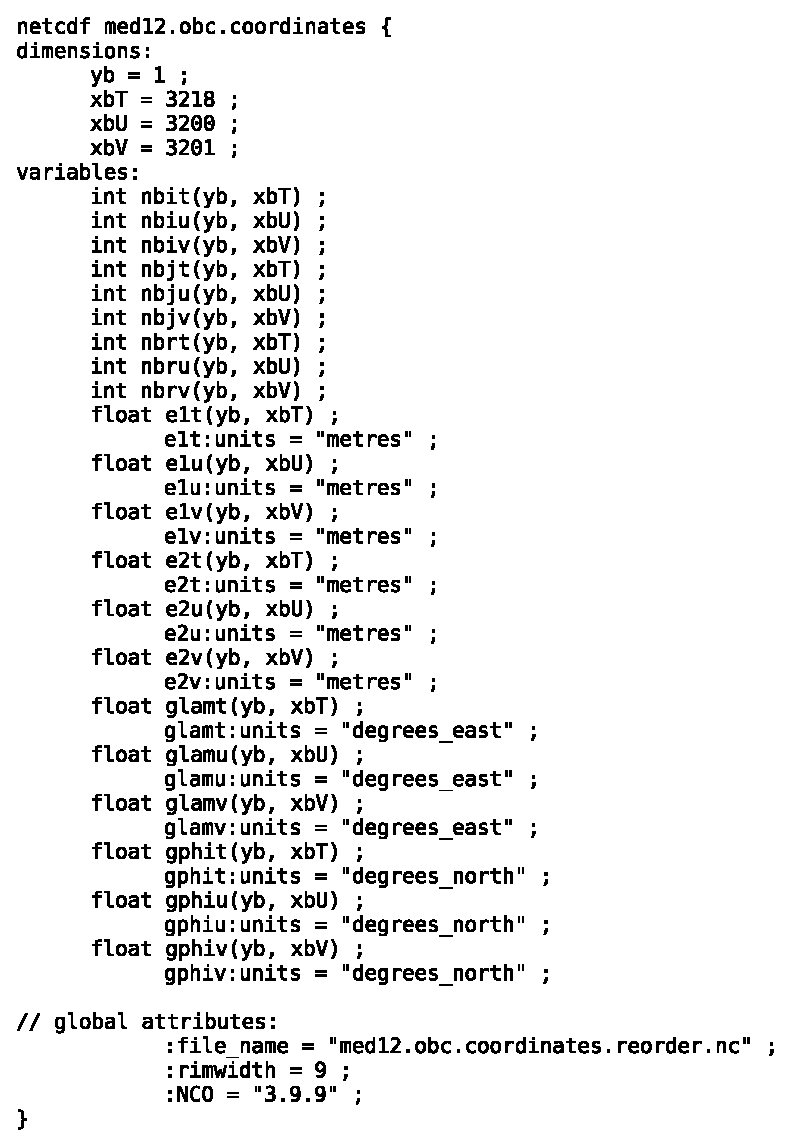
\includegraphics[width=1.0\textwidth]{Fig_LBC_nc_header}
\caption {     \protect\label{fig:LBC_nc_header} 
Example of the header for a \protect\ifile{coordinates.bdy} file}
\end{center}   \end{figure}
%>>>>>>>>>>>>>>>>>>>>>>>>>>>>

%----------------------------------------------
\subsection{Volume correction}
\label{subsec:BDY_vol_corr}

There is an option to force the total volume in the regional model to be constant, 
similar to the option in the OBC module. This is controlled  by the \np{nn\_volctl} 
parameter in the namelist. A value of \np{nn\_volctl}\forcode{ = 0} indicates that this option is not used. 
If  \np{nn\_volctl}\forcode{ = 1} then a correction is applied to the normal velocities 
around the boundary at each timestep to ensure that the integrated volume flow 
through the boundary is zero. If \np{nn\_volctl}\forcode{ = 2} then the calculation of 
the volume change on the timestep includes the change due to the freshwater 
flux across the surface and the correction velocity corrects for this as well.

If more than one boundary set is used then volume correction is
applied to all boundaries at once.

\newpage
%----------------------------------------------
\subsection{Tidal harmonic forcing}
\label{subsec:BDY_tides}

%-----------------------------------------nambdy_tide--------------------------------------------
\forfile{../namelists/nambdy_tide} 
%-----------------------------------------------------------------------------------------------

Options are defined through the  \ngn{nambdy\_tide} namelist variables.
 To be written....




\end{document}
